\documentclass{article}

% to give various notational syntax
\usepackage{amsmath,amsthm,amssymb, mathtools, enumerate, physics}

% for including images
\usepackage{graphicx}
\graphicspath{ {../../Images/} }
% Resize figures that are too wide for the page.
\makeatletter
\def\ScaleIfNeeded{%
  \ifdim\Gin@nat@width>\linewidth
    \linewidth
  \else
    \Gin@nat@width
  \fi
}
\makeatother
\let\oldincludegraphics\includegraphics
\renewcommand\includegraphics[2][]{%
  \oldincludegraphics[width=\ScaleIfNeeded]{#2}
}
%
%% for bibliography and citation
%\usepackage[square,compress]{natbib}
%\setcitestyle{super,comma}
%\bibliographystyle{unsrtnat}
%
%% for executing and including python code
%\usepackage{pythontex}
%
%% for defining lovely colors
%\usepackage{xcolor}
%\definecolor{light-gray}{gray}{0.95}
%
%% for syntax highlighting of non-python languages
%\usepackage{minted}
%\usemintedstyle[cpp]{manni}
%\newcommand{\cpp}[1]{\mintinline{cpp}{#1}}

% for linking sections of the document and table of contents
\usepackage{hyperref}
\hypersetup{
    colorlinks=true, %set true if you want colored links
    linktoc=all,     %set to all if you want both sections and subsections linked
    linkcolor=blue,  %choose some color if you want links to stand out
}


\newcommand{\nn}{\newline\newline}
\newcommand{\n}{\newline}
\newcommand{\bq}{\begin{equation}}
\newcommand{\eq}{\end{equation}}
\newcommand{\ba}{\begin{align}}
\newcommand{\ea}{\end{align}}
\newcommand{\bi}{\begin{itemize}}
\newcommand{\ei}{\end{itemize}}
\newcommand{\ct}[1]{\citep{#1}}

\newcommand*{\Perm}[2]{{}^{#1}\!P_{#2}}
\newcommand*{\Comb}[2]{{}^{#1}C_{#2}}




\begin{document}

\title{Bayesian Data Analysis}
\date{}
\maketitle

\textbf{Question:} Within the decision theoretic framework for data analysis, define estimation and estimators, and give the two most common subtypes of estimation.
\nn

\textbf{Question:} Define \emph{likelihood} and describe the \emph{Maximum Likelihood Estimation} decision procedure.
\n
\textbf{Problem:} What is the form of MLE for $n$ i.i.d. draws with a model that each $X \sim N(\theta, 1)$? What about if instead $X \sim \mathrm{DoubleExp}(\theta)$?
\nn

\textbf{Question:} Describe the \emph{least square fitting} decision procedure; Under what conditions is it also the MLE decision procedure?
\n

\textbf{Question:} How is maximizing L2-penalized log likelihood (a common decision procedure) equivalent to a Bayesian Maximum a Posteriori decision procedure?
\n

\textbf{Question:} Describe the data generating mechanism and corresponding likelhood function for binary classification with \emph{Logistic Regression}.

\textbf{Question:} Give a geometric picture for the data generating mechanism and LSQ fitting procedure for \emph{Linear Regression}.

\vspace{.3 in}
\tableofcontents

\section{Review of Estimators Within the DTFoA}
\textbf{If actions and  truths are represented by the same space, that space being the set of possible true data generating mechanisms defined by the model, the analysis is called \emph{estimation}.}  This is because the mathematical description of the data generating mechanism is in terms of some number of parameters, so the analysis is seeking to estimate values of these parameters. There are two common instantiations of this:
\begin{enumerate}
\item \textbf{Density estimation}, where your data is a set of draws from a population, and your truths/actions are forms of the underlying population probability density.
\item \textbf{Function estimation}, where your data is a set of variable tuples, like $(X_1, X_2, X_3, Y)$, and your truths/actions are functional relationships between the variables.
\end{enumerate}

In the former kind of analysis you seek to estimate the values of the parameters of the distribution, in the latter the parameters of the function. The possible densities or functions under consideration are those defined by your choice of model. Note that the functions are stochastic (if your model was deterministic then you would be able to get the parameter values by direct calculation from your data points!). 
\newline

\textbf{ An \emph{estimator} is simply a decision rule used in estimation type analyses.} In function estimation, because our truths are stochastic, we are essentially seeking to estimate conditional densities e.g. the distribution of $Y$ given $\{X_i\}$. Thus in function estimation your model class will be a set of families of conditional distributions. In almost all cases function estimation is concerned with writing one of the variables as an explicit function of the others like $Y = f(X_1, X_2, X_3, \vec{\Theta})$, where $\Theta$ is a vector of unmeasured parameters. The most common application of this is to predict future $Y$s based on future measurements of the $X$s. In this case function estimation conveniently breaks down into two cases: 
\begin{enumerate}
\item \textbf{categorical estimation (logistic regression)}, where $Y$ is a discrete categorical variable.
\item \textbf{regression}, where $Y$ is a continuous function of $X$s.
\end{enumerate}

In general terms \textbf{a statistic, $\delta(\vec{X})$, is any computable function of the data}, so an estimator is a statistic that we use to make our estimate of parameter value. Given some model for the data generating mechanism, a statistic has a \textbf{sampling distribution which describes the distribution of the computed value of the statistic given some value for the parameter of the data-generating distribution.} When a statistic is serving as an estimator, the sampling distribution for the statistic is the same as the distribution over actions of an estimator. 
\n


\section{Maximum Likelihood Estimators}
\textbf{The likelihood, $L(\theta)$, is a function of the parameter parameterizing the true data-generating distribution ($\theta$) which gives the probability of the observed data ($\vec{X}$)being caused by that underlying generating distibution.}
\begin{align*}
L(\theta) = f(\vec{X}|\theta).
\end{align*}

Recall that an estimator is just a decision procedure (DP) within the DTFoA - it is an algorithm that takes in the data and uses it to choose one action. In the case of estimation DPs the actions are choosing a representative distribution from the model which we will move forward with for the purposes of prediction or interpretation. \textbf{The Maximum Likelihood Estimator (MLE) is thus a particular DP of the esimation variety. It is the algorithm which says: take the data, use it to compute the likelihood $L(\theta)$ for the different possible truths in the chosen model, then select the $\theta$ which gives the maximum likelihood for the observed data.} For many models, once th likelihood is written down analytically it becomes clear what statistic on the data will satisfy this definiton. In other cases the best approach is just to numerically calculate the likelihood on a dense grid of the truths and maximizing point from that grid. 
\newline

For data that consists of i.i.d. points, the likelihood can always be written as a product of the likelihoods for each individual point:
\begin{align*}
L(\theta) = f(\vec{X}|\mu) = \prod_i f(\vec{X_i}|\mu).
\end{align*}

\subsection{Problem: MLE for Normal I.I.D. Sample}
For instance for $n$ i.i.d. draws with a model that each $X \sim N(\mu, 1)$ we can see that since $f(X) \propto e^{(X-\mu)^2}$ we will have $L(\mu) \propto e^{\Sigma (X_i-\mu)^2}$. So the form of the MLE for this system will be a statistic (function of the data) which minimizes $\Sigma (X_i-\mu)^2$. Actually we know such a statistic: the definition of the sample mean is that it is the number that will minimize the sum of squared distances from itself to all the points in the sample. If this is difficult to see then try expanding out $\mathrm{E}\big[(X-\alpha)^2\big]$.
\n

What about if instead the model is a centered double exponential distribution: $f(X) = e^{(|X-\mu|}$? In this case the MLE will be the statistic which minimizes $\Sigma |X_i-\mu|$. You can convince yourself that actually the statistc that does this by definition is the median.
\n

MLEs generally do well, especially asymptotically. But  note that \textbf{sometimes even if your model doesn't contain the true form of the generating distribution, you can still get a likelihood function which is relatively peaked}. That is why it is important to use a suitably large model and to compare actual values for the likelihood probabilities.

\subsection{Least-Squares Fitting and MLEs}
A common decision procedure for function estimation is to choose a $\theta$ which minimizes the sum of squared distances between the actual observed $Y$ values and the corresponding predicted $Y = f(X; \theta)$ values. This \textbf{Least Squares Fitting} does have some intuitive appeal, but it is also has some support on the basis of MLE. In many systems a very good model is that $Y$ is a deterministic function of $X$ plus some random noise about zero: $Y = f(X; \theta) + \epsilon$ where $\epsilon \sim N(0, \sigma_0)$. For such models the function (conditional distributions) that we seek to estimate will be a normal distribution. The likelihood for the data will be a product of normal distributions, and maximizing the likelihood will involving minimizing the term in the exponent:
\begin{align*}
L(\theta) \propto \prod_i e^{-(f(\vec{X}_i; \theta)-Y_i)^2/\sigma_0^2}
\end{align*}
This term will be proportional to the sum of squared differences between the predicted and observed $Y$ values. \textbf{So for such models, $Y = f(X; \theta) + \epsilon$, least-squares fitting is in fact the MLE.}

\subsection{Penalized log MLE (Backdoor Bayesianism)}
Here is an interesting relationship between Bayesian decision procedures and maximum likelihood procedures. Consider taking the log of the Bayesian posterior density:
\begin{align*}
f(\theta | \vec{X}) = \frac{f(\vec{X}|\theta)f(\theta)}{f(\vec{X})}\\
\implies \log{f(\theta | \vec{X})} = \log{L(\theta)} + \log{f(\theta)} - \log{f(\vec{X})}.
\end{align*}
Here $f(\vec{X})$ will be some number for your particular data (and prior), it does not depend on the value of $\theta$. A common estimation procedure is to maximize log likelihood subject to some correction term, like a penalty for model complexity or a regularization term that drives the selection toward some specific choice. This kind of procedure can sometimes be interpreted as doing a Maximum A Posteriori (MAP) decision procedure with a certain prior. For example L2 regularization uses a term which drives the selection to $\theta_0$ by a penalty of $(\theta-\theta_0)^2$. In this case maximimizing the penalized log likelihood is equivalent to MAP with a Gaussian prior. If the penalty term doesn't integrate to one when exponentiated then it isn't a true prior, but you might still interpret this as adding in a prior to the decision procedure, but giving it a different weight than the standard Bayesian approach. 

\section{Logistic Regression}
Logistic regression is a method for classification (predicting categorical response variables) in which you seek a function that for the probability of $Y_i$ to be in each category given it's corresponding $X_i$ (which is a random vector). This is a function estimation problem, and for a binary classification the model is $Y_i \sim Bernoulli(f(X_i; \theta))$. This model can be interpreted as capturing our belief that there are other unmeasured variables that will cause an ensemble of universes with identical $X_i$ to give rise to different values of $Y_i$ in a proportion given by the probability. 
\n

Typically the argument of $f(X; \theta)$ has the form of a linear model (meaning linear in the parameters $\theta$) i.e. f = $f(X\cdot \theta)$. The random vector $X$ can contain the measured independent variables but also any arbitrary transformations of those variables. For instance, if we have real measured independent variables $X_1$ and $X_2$, our first pass might be $f(\theta_1X_1 + \theta_2X_2)$.  If this didn't give a suitable fit to the data we could try the more complex $f(\theta_1X_1 + \theta_2X_2 + \theta_3X_1^2 + \theta_4X_2^2)$. Besides choosing how to construct this linear argment it is also necessary to stipulate the functional form of $f$,for which there are some common choices. The constraint is that it must map all the possible inner product values to outputs on [0,1]. 
\n

Finally, the full model must be fitted with the data in order to estimate the $\theta$s - this is often done with MLE. Let $z = f(X; theta)$, since $Y$ is Bernoulli (taking value 1 with probability $z$ or 0 with probability $1-z$) the likelihood for a single $(X_i, Y_i)$ pair is
\begin{align*}
L = z^Y (1-z)^{(1-Y)},
\end{align*}
where the $\theta$ dependence of $L$ and $z$ has been suppressed. For $n$ i.i.d. observations the full $L(\theta)$ is the product, but there is no closed form solution for the maximizer of such a thing, so it is handled numerically. Note that in logistic regression there is not much emphasis on the $f(X; \theta)$ being somehow a representation of a real physical generating mechanism, and typically no interpretation given to the $\theta$s, so often this is used like a machine learning technique. 


\section{Linear Regression}
Assume you have data points of the form $(x, y)$. You can think of the list of $x$'s as a vector in $\cal{R}_n$ and the list of corresponding $y$ values likewise. In linear regression you are modeling each $y$ by $y = ax+b$, so you can capture this over your whole data set with a vector relationship $\vec{y} = a\vec{x}+b\vec{1}$. Your model prediction of $\vec{y}$ is a point in $\cal{R}_n$ and this formula says that this point must lie in the plane spanned by $\vec{x}$ and $\vec{1}$, the exact point depending on the constants $a$ and $b$.
\newline

In this geometric picture, to say that we want to choose the $a$ and $b$ according to LSQ fitting (minimizing sum of squared distances between true and predicted $y$-values) is to say that we want to our predicted vector, $\hat{y}$, as close as possible in euclidean distances to the point real point, $\vec{y}$ , in $\cal{R}_n$. Since we know $\hat{y}$ can be any point from the prescribed plane spanned by $\vec{x}$ and $\vec{1}$ we can see that the closest point we can choose is the orthogonal projection of the true $\vec{y}$ onto this plane. This orthogonal projection is a quantity that we can write an expression and ``solve for'' obtaining an analytical expression for this best-in-the-LSQ-sense $\hat{y}$ in terms of the $\vec{x}$ and $\vec{y}$.

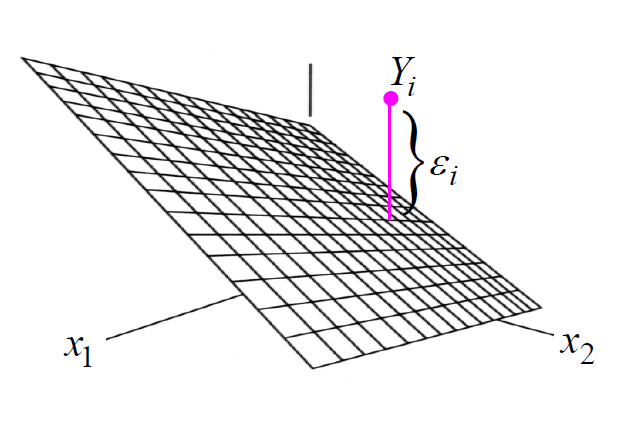
\includegraphics{geometry-regression} 

To actually do this math starts by finding a new orthonormal basis for the plane that $\hat{y}$ lives in. I won't go into it here. The punchline is that the "equation" for our best-in-the-LSQ-sense choice (prediction closest in euclidean distance to true values) can be cast in terms of the sample variances of $x$ and $y$, and the sample correlation $\rho$. 

\subsection{Multiple Linear Regression}
In this case there are multiple independent variables ($x$'s) that can be used to explain the $y$'s and the model can include "interaction terms" of the form $x_ix_j$. A good example is a data set of salary as a function of gender and years of experience. 


\end{document}